\documentclass{Alexandre}
\usepackage[portuguese, ruled, linesnumbered]{algorithm2e}
\usepackage{multirow}
\usepackage{multicol}
\usepackage{color}
\usepackage{diagbox}
\usepackage{setspace}
\usepackage{listings}
\usepackage{color}
\usepackage{caption}
\usepackage{mwe}
\usepackage[normalem]{ulem}
\usepackage[framemethod=tikz]{mdframed}

\definecolor{codegreen}{rgb}{0,0.6,0}
\definecolor{codegray}{rgb}{0.5,0.5,0.5}
\definecolor{codepurple}{rgb}{0.58,0,0.82}
\definecolor{backcolour}{rgb}{0.95,0.95,0.92}

\lstdefinestyle{mystyle}{
  backgroundcolor=\color{backcolour},   commentstyle=\color{codegreen},
  keywordstyle=\color{magenta},
  numberstyle=\tiny\color{codegray},
  stringstyle=\color{codepurple},
  basicstyle=\footnotesize,
  breakatwhitespace=false,         
  breaklines=true,
  captionpos=b,                   
  keepspaces=true,                 
  numbers=left,                    
  numbersep=5pt,                  
  showspaces=false,                
  showstringspaces=false,
  showtabs=false,                  
  tabsize=2
}

\setbeamertemplate{bibliography item}[triangle]

\title{Democracia Eletrônica}
\author{Alexandre Mendonça Fava\inst{1}}


\institute[UDESC]{
  \newline \newline \newline
  \inst{1}
  Mestrado Acadêmico em Computação Aplicada - PPGCA
}

\date{6 Setembro 2019}

\subject{}

\logo{

\includegraphics[scale=0.8]{Figuras/Logo-UDESC.jpg}
}

\begin{document}


\begin{frame}
  \titlepage
\end{frame}
%[Transparência 1] Bom dia a todos. Por questões de formalidade, meu nome é Alexandre Mendonça Fava.


\begin{frame}{AGRADECIMENTOS}

    O presente trabalho foi realizado com apoio da Coordenação de Aperfeiçoamento de Pessoal de Nível Superior - Brasil (CAPES) - Código de Financiamento 001. 

\end{frame}
%[Transparência 2] Destaco que o presente trabalho sobre a Democracia Eletrônica foi realizado com total apoio da CAPES.


\begin{frame}{SISTEMAS COLABORATIVOS}
    \begin{center}
        \textbf{Capítulo 7}
    \end{center}
    \begin{figure}
        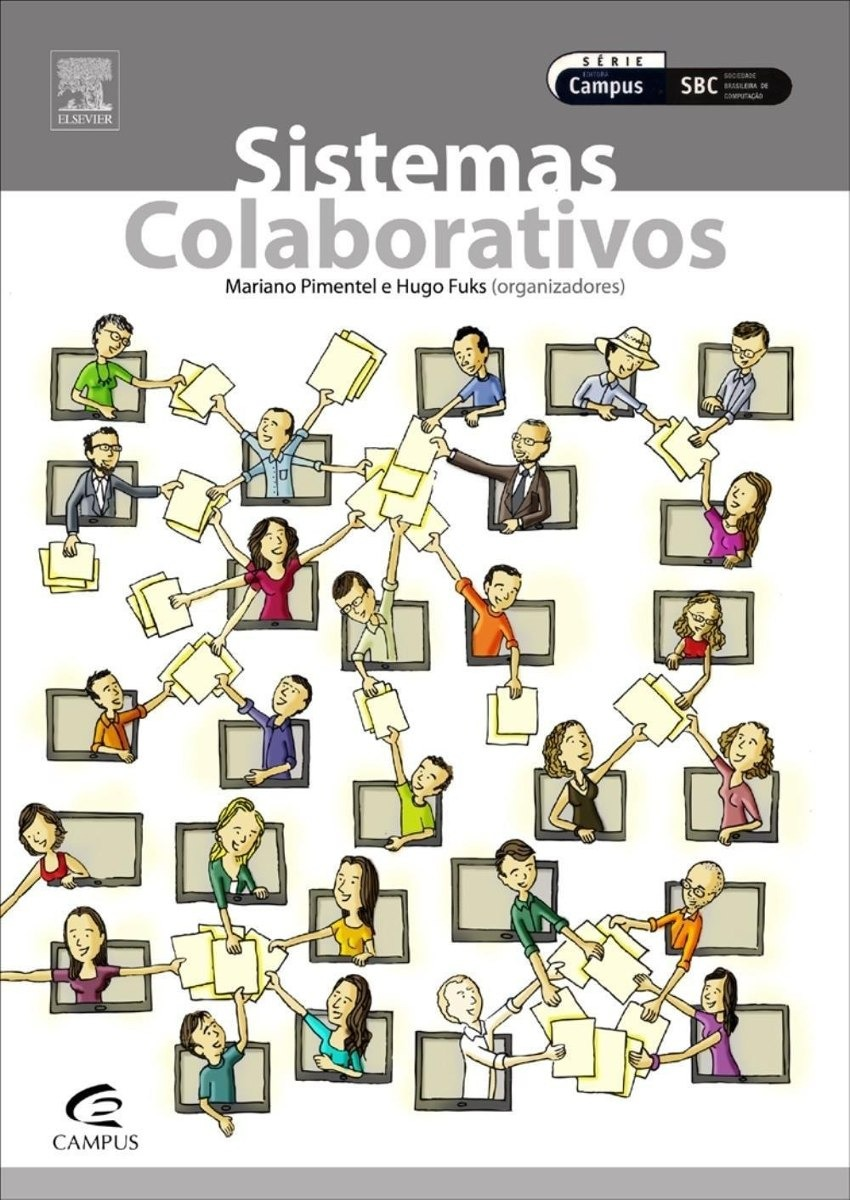
\includegraphics[scale = 0.15]{Figuras/Livro-SistemasColaborativos.jpg}
    \end{figure}

\end{frame}
%[Transparência 3] Para situá-los, a Democracia Eletrônica é o sétimo capítulo do livro de Sistema Colaborativos, capítulo esse que fora escrito pela: Renata Mendes de Araujo; Claudia Cappelli; Bruna Diirr; Priscila Engiel; e pelo Rafael Lage Tavares.


\begin{frame}{SISTEMAS COLABORATIVOS}
    
    \begin{center}
        \Large  Democracia Eletrônica
    \end{center}
    
\end{frame}
%[Transparência 4] Juntos, eles escreveram sobre a Democracia Eletrônica, a qual para eu poder explicá-la nessa apresentação eu preciso primeiramente, destrinchar os seus dois conceitos fundamentais: Democracia e Eletrônica.


\begin{frame}{DEMOCRACIA}
    \begin{center}
        \Large \textbf{Demo + Cracia}
        
        \Large Povo + Poder
    \end{center}

\end{frame}
%[Transparência 5] A Democracia de acordo com o próprio livro, é uma palavra que vem do grego e que agrega dois significados distintos, onde ‘demo’ significa “povo” e ‘cracia’ significa “poder”.


\begin{frame}{DEMOCRACIA}

    \begin{center}
        \Large O Poder do Povo
    \end{center}

\end{frame}
%[Transparência 6] Ou seja: poder do povo.


\begin{frame}{DEMOCRACIA}

    \begin{center}
        \Large Todo o poder emana do povo
    \end{center}

\end{frame}
%[Transparência 7] O que me faz lembrar do primeiro artigo da nossa amada constituição, onde está dito: “Todo o poder emana do povo.”


\begin{frame}{DEMOCRACIA}

    \begin{center}
        \Large Todo o poder emana do povo,
        
        \vspace{2cm}
        
        \Large que o exerce por meio de representantes eleitos ou diretamente
    \end{center}

\end{frame}
%[Transparência 8] Entretanto; isso não é tão verdade assim...
%Pois a nossa constituição não se resume a dizer APENAS que todo o poder emana do povo, mas também que: o povo exerce esse poder “por meio de representantes eleitos ou diretamente.”



\begin{frame}{DEMOCRACIA REPRESENTATIVA}

    \begin{center}
        \Large Todo o poder emana do povo,
        
        \vspace{2cm}
        
        \Large que o exerce por meio de \textbf{representantes eleitos} ou diretamente
    \end{center}

\end{frame}
%[Transparência 9] Com isso, é possível notar que existem duas formas de democracia aqui. A primeira é a qual o povo exerce seu poder por meio de representantes eleitos, também chamada de democracia representativa ou democracia indireta.


\begin{frame}{DEMOCRACIA DIRETA}

    \begin{center}
        \Large Todo o poder emana do povo,
        
        \vspace{2cm}
        
        \Large que o exerce por meio de representantes eleitos ou \textbf{diretamente}
    \end{center}

\end{frame}
%[Transparência 10] Já a segunda é a qual o povo exerce seu poder diretamente, também chamada de democracia direta ou participativa.


\begin{frame}{DEMOCRACIA SEMIDIRETA}

\end{frame}
%[Transparência 11] Ou seja, o Brasil, constitucionalmente, possui os dois tipos de democracia. O que o enquadra como uma democracia semidireta. Que nada mais é que a união das duas formas de democracia.


\begin{frame}{DEMOCRACIA SEMIDIRETA}

    \begin{figure}
        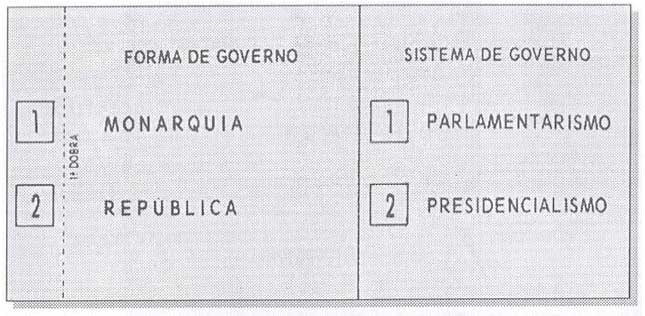
\includegraphics[scale = 0.21]{Figuras/Plebiscito1993.jpg}
        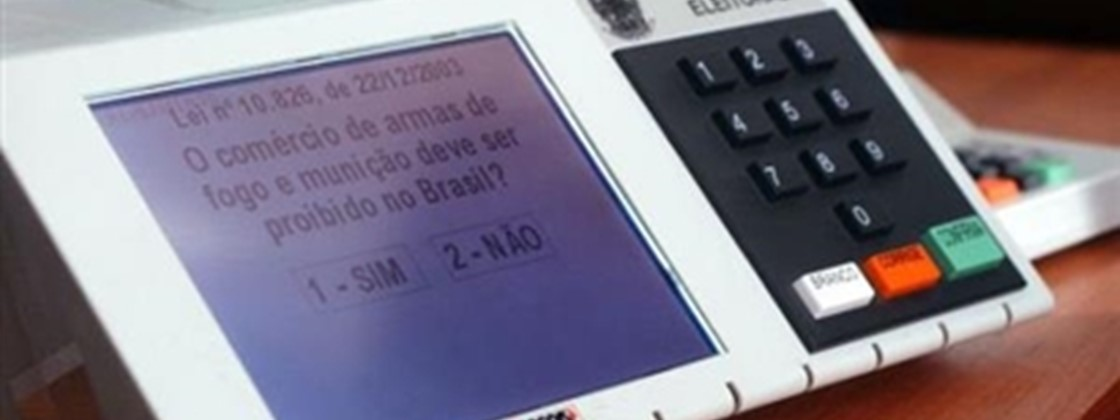
\includegraphics[scale = 0.20]{Figuras/Referendo2005.jpg}
    \end{figure}

\end{frame}
%[Transparência 12] Entretanto; isso não é tão verdade assim...
%Isso, pois historicamente em âmbito nacional o povo brasileiro participou APENAS de duas decisões relacionadas a esfera política. 
%A primeira, em 1993, onde o povo decidiu o tipo de governo [imagem da esquerda].
%E a segunda em 2005, onde o povo decidiu sobre a venda de armas no Brasil [imagem da direita]. 
%Eu não sei vocês, mas com esse histórico de participação popular, eu não diria que ‘Todo poder emana do povo diretamente’. Por isso que não minha humilde opinião, embora teoricamente o Brasil seja uma democracia semidireta, tecnicamente o Brasil é muito mais uma democracia indireta. 

\begin{frame}{DEMOCRACIA SEMIDIRETA}

    \begin{figure}
        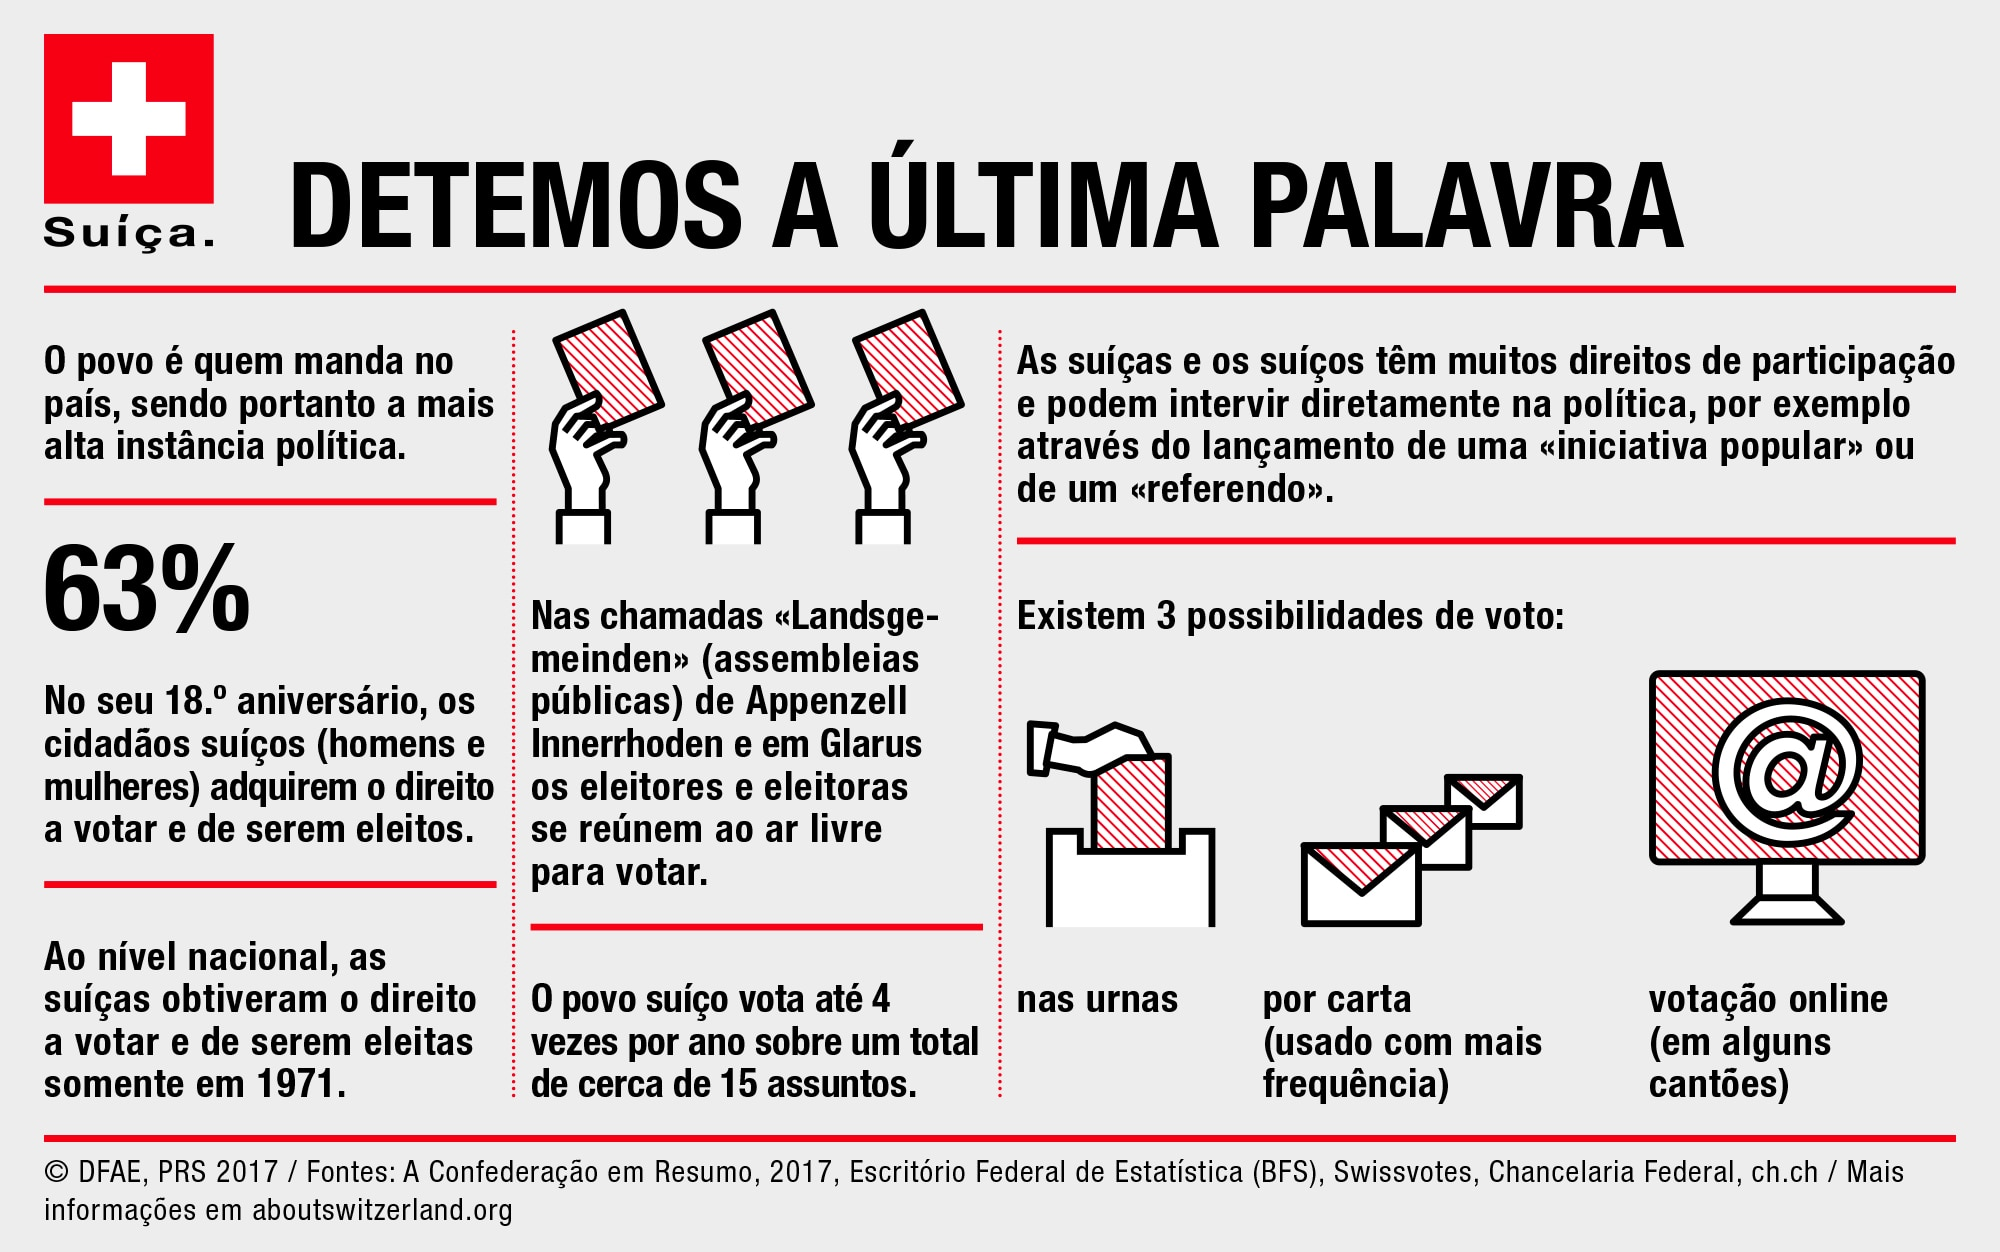
\includegraphics[scale = 0.14]{Figuras/Suica.jpg}
    \end{figure}

\end{frame}
%[Transparência 13] Democracia semidireta, a meu ver, é a Suíça. Lá o povo é quem manda no país, sendo portanto, a mais alta instância política. Os suíços por exemplo têm total poder para intervir diretamente na política seja por iniciativas populares ou por referendos. Os meios mais comuns usados nesse sentido são as urnas, cartas, ou votações online.


\begin{frame}{ELETRÔNICA}

\end{frame}
%[Transparência 14] E falando de votações online, isso me ajuda a introduzir o segundo conceito da Democracia Eletrônica. A eletrônica. Eletrô, vem de elétrons (âmbar do grego), corrente. Ica, significa ciência, técnica. Assim como a Gramática é a Ciência das letras, a Eletrônica seria a Ciência dos Elétrons ou a Técnica dos Elétrons. 


\begin{frame}{ELETRÔNICA}

    \begin{figure}
        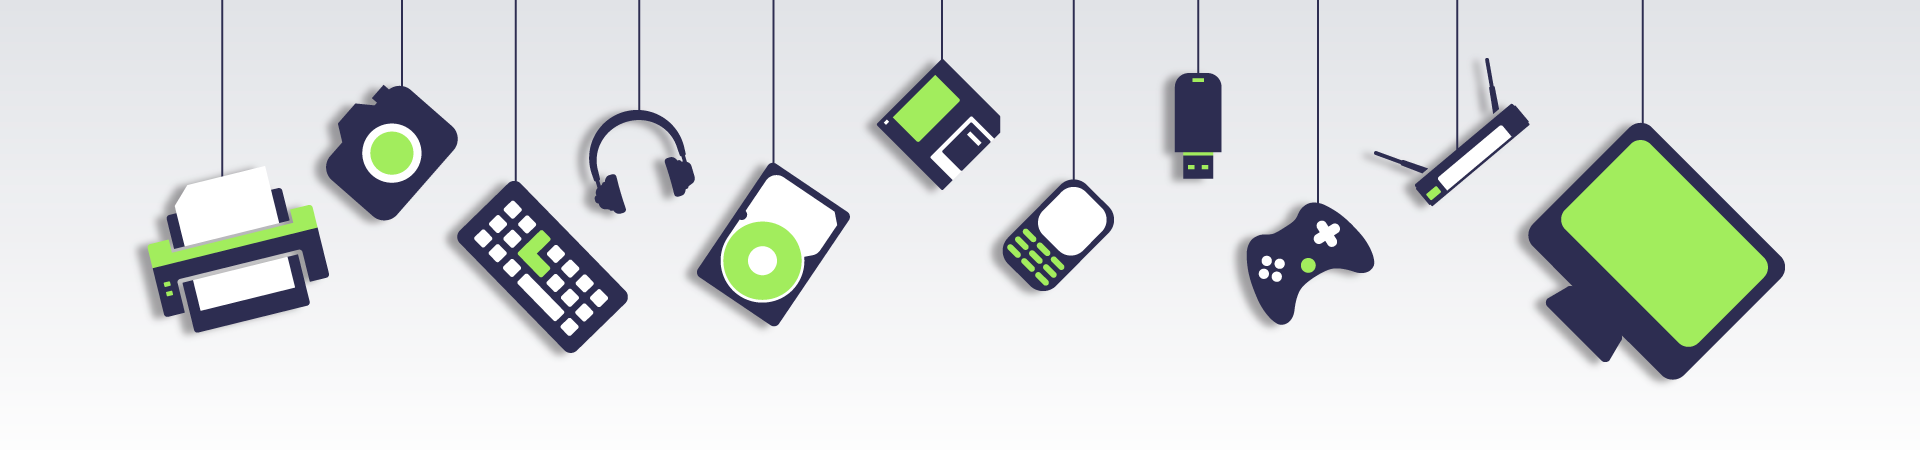
\includegraphics[scale = 0.20]{Figuras/Eletronicos.png}
    \end{figure}

\end{frame}
%[Transparência 14] Que traduzindo são os computadores, os celulares, e todos os demais aparelhos do gênero. Ou seja, a Democracia Eletrônica, nada mais é, do que uma democracia dada por via dos meios eletrônicos.


\begin{frame}{DEMOCRACIA ELETRÔNICA}

    Qual democracia?

\end{frame}
%[Transparência 14] Mas a pergunta que fica é: mas qual democracia?


\begin{frame}{DEMOCRACIA ELETRÔNICA}

    Qual democracia? R: Democracia Direta.

\end{frame}
%[Transparência 14] Notoriamente, a democracia direta, até porque ela é a mais democrática das democracias! Mas se ela é a mais democrática das democracias, por que não temos uma Democracia Direta? E a resposta é basta simples, é porque ela é impossível.


\begin{frame}{DEMOCRACIA IMPOSSÍVEL}

    \begin{figure}
        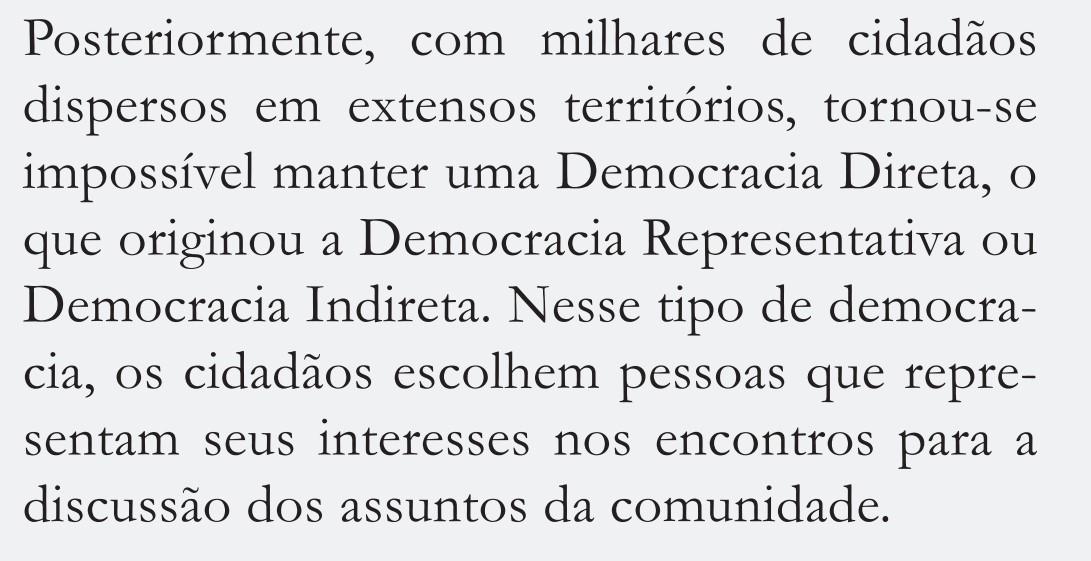
\includegraphics[scale = 0.35]{Figuras/Democracia-Impossivel.jpg}
    \end{figure}

\end{frame}
%[Transparência 14] A grande quantidade populacional e a larga extensão territorial, tornaram “impossível manter uma Democracia Direta.”


\begin{frame}{DEMOCRACIA \sout{IMPOSSÍVEL}}

    \begin{figure}
        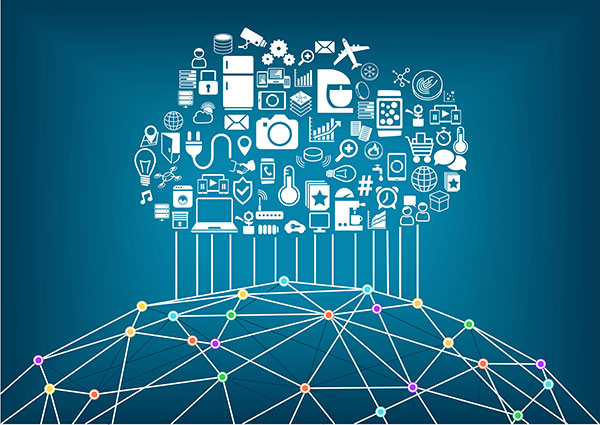
\includegraphics[scale = 0.40]{Figuras/Internet.jpg}
    \end{figure}

\end{frame}
%[Transparência 14] Quer dizer... Era impossível, com os adventos dos eletrônicos e da grande rede de computadores, surgiu novamente a possibilidade de uma democracia direta. 


\begin{frame}{DEMOCRACIA ELETRÔNICA}

\end{frame}
%[Transparência 14] Ou melhor dizendo... Uma democracia eletrônica. 


\begin{frame}{DEMOCRACIA ELETRÔNICA}

    \begin{center}
        Governo Eletrônico
    \end{center}
    \vspace{3cm}

\end{frame}
%[Transparência 14] E para que haja uma democracia eletrônica, é NECESSÁRIO antes ter um Governo Eletrônico. Sendo um governo eletrônico, nada mais que um governo que se utiliza da ‘internet para prestar serviços e entregar informações aos cidadãos’. Dito isso eu pergunto: O Brasil é um governo eletrônico? Claro que é, existem os sites do governo, dos estados, dos municípios, além dos inúmeros serviços que o governo presta. Uma pergunta mais pertinente seria: Quanto eletrônico é o governo brasileiro? 


\begin{frame}{DEMOCRACIA ELETRÔNICA}

    \begin{center}
        Governo Eletrônico
    \end{center}
    \begin{figure}
        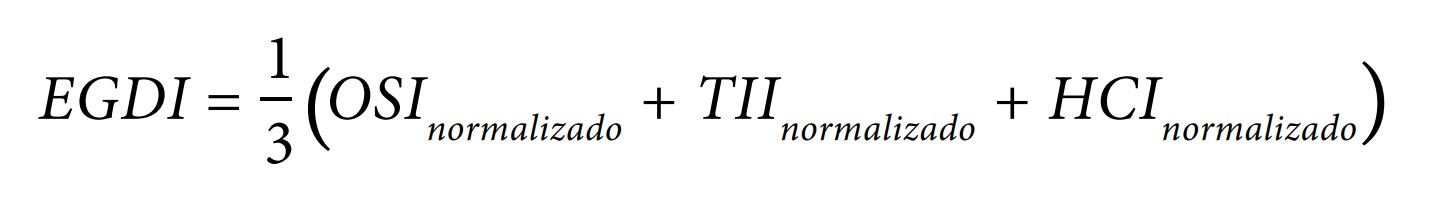
\includegraphics[scale = 0.30]{Figuras/EGDI.jpg}
    \end{figure}

\end{frame}
%[Transparência 14] E sim, existe uma forma de medir o nível de governo eletrônico de um país. Na verdade, não existe uma forma, mas sim uma fórmula. Essa fórmula eu tirei de um Estudo Sobre Governo Eletrónico realizada em 2018 pela Organização das Nações Unidas. Essa fórmula mede mais especificamente o Índice de Desenvolvimento de Governo Eletrônico, e para isso ela se utiliza de três variáveis (as quais oscilam de zero até um):
%OSI: que é o Índice de Serviços Online.
%TII: que é o Índice de Infraestrutura de Telecomunicações.
%HCI: que é o Índice de Capital Humano. 


\begin{frame}{Índice de Serviços Online}

    \begin{itemize}
        \item Presença de uma aplicação móvel para fornecer serviços de governo eletrônico
        \item Informações sobre o orçamento nacional ou a política orçamenta
        \item Presença de uma política sobre dados governamentais abertos
        \item Presença de recursos relativos à acessibilidade
        \item Presença de um mapa do site
    \end{itemize}

\end{frame}
%[Transparência 14] O OSI mede por exemplos os seguintes itens: 
%Presença de uma aplicação móvel para fornecer serviços de governo eletrônico
%Informações sobre o orçamento nacional ou a política orçamenta
%Presença de uma política sobre dados governamentais abertos
%Presença de recursos relativos à acessibilidade
%Presença de um mapa do site


\begin{frame}{Índice de Serviços Online}

    \begin{figure}
        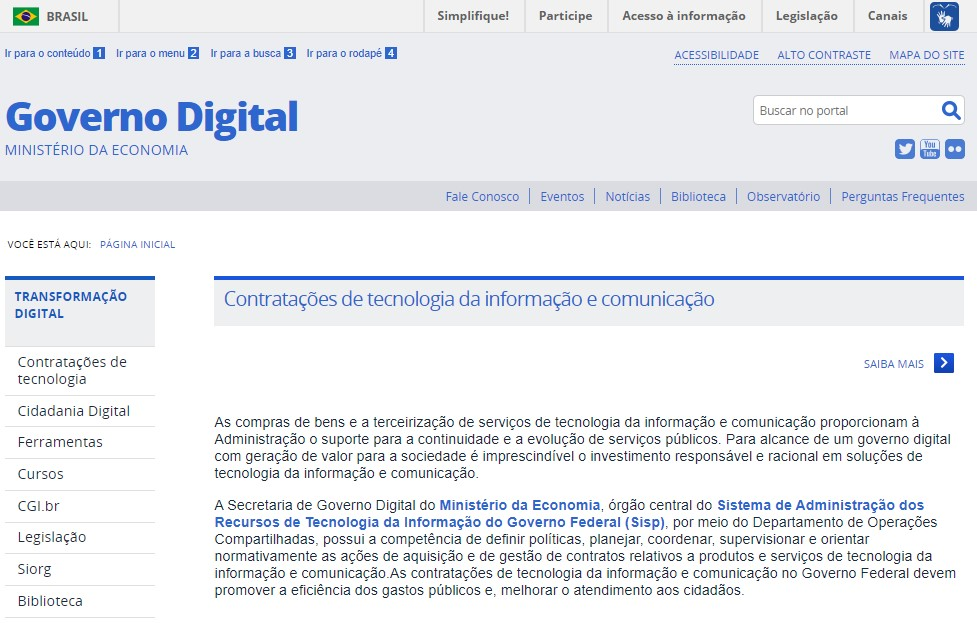
\includegraphics[scale = 0.38]{Figuras/GovernoDigital.jpg}
    \end{figure}

\end{frame}
%[Transparência 14] No que diz respeito a índices orçamentários, prestação de serviços, prestação de contas o Brasil não deixa a desejar, o Brasil inclusive tem um sítio intitulado Governo Digital: https://www.governodigital.gov.br/
%O problema do Brasil não é o OSI, a nota do Brasil inclusive nesse aspecto é 0,9236. Onde o Brasil peca mesmo é no TII e no HCI.


\begin{frame}{Índice de Infraestrutura de Telecomunicações}

    \begin{figure}
        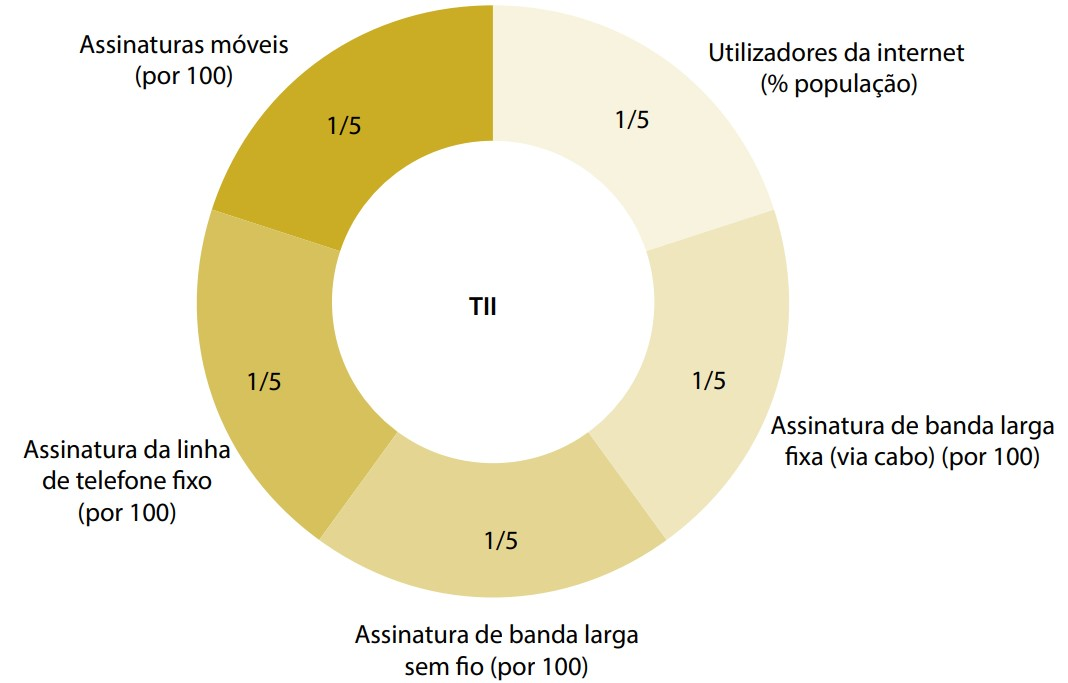
\includegraphics[scale = 0.30]{Figuras/TII.jpg}
    \end{figure}

\end{frame}
%[Transparência 14] Acredito que nem preciso dizer o quanto a infraestrutura do Brasil é precária. Com a Internet chegando apenas ¾ da população brasileira. Isso dá mais de 50 milhões de brasileiros sem acesso a internet. O que gera para nós um TII  de 0,5220.


\begin{frame}{Índice de Capital Humano}

    \begin{figure}
        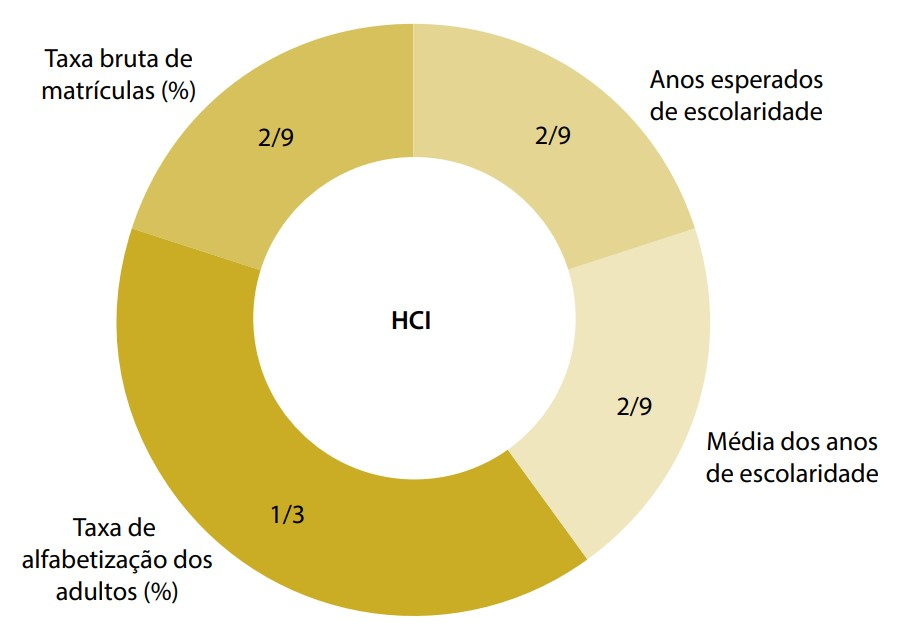
\includegraphics[scale = 0.30]{Figuras/HCI.jpg}
    \end{figure}

\end{frame}
%[Transparência 14] Isso sem mencionar o HCI. Que nada mais é do que a capacitação dos cidadãos em acessar e interpretar alguma informação ou serviço prestado pelo governo. Até porque não adiante o cidadão ter toda a infraestrutura necessário, o governo apresentar todas as informações e o cidadão não saber interpretar aquelas informações ou não saber deliberar sobre as melhores ações. É aqui é o alto analfabetismo do Brasil pesa com os seus mais de 11 milhões de analfabetos, isso sem mencionar a baixa escolaridade do povo brasileiro. O que resulta em um HCI que não passa de 0,7525.


\begin{frame}{Índice de Desenvolvimento do Governo Eletrônico}

    EGDI =  1/3 (0,9236 + 0,5220 + 0,7525)
    
    \vspace{1cm}
    
    EGDI = 0,7327

\end{frame}
%[Transparência 14] Somando tudo na fórmula, o Brasil tem um EGDI de 0,7327. Ou seja, a nota do governo eletrônico do Brasil é 7,3. Mas o que isso reflete de fato na Democracia Eletrônica? E a resposta é bastante simples, isso reflete nos níveis de participação democrática. 


\begin{frame}{NÍVEIS DE PARTICIPAÇÃO DEMOCRÁTICA}

    \begin{enumerate}
        \item Prestação de Serviços 
        \item Coleta de Opinião Pública 
        \item Prestação de Contas 
        \item Democracia Deliberativa 
        \item Democracia Direta
    \end{enumerate}

\end{frame}
%[Transparência 14] Em resumo, uma das classificações de Democracia Eletrônica a define em cinco níveis:
%1-) Prestação de Serviços 
%2-) Coleta de Opinião Pública 
%3-) Prestação de Contas 
%4-) Democracia Deliberativa 
%5-) Democracia Direta


\begin{frame}{NÍVEL ATUAL}

    \begin{figure}
        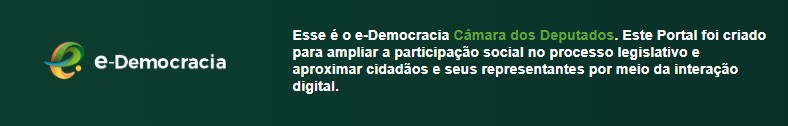
\includegraphics[scale = 0.50]{Figuras/eDemocracia.jpg}
    \end{figure}
    \begin{center}
        \url{https://edemocracia.camara.leg.br/}
    \end{center}

\end{frame}
%[Transparência 14] Atualmente existe um sítio onde os cidadãos podem: fazer perguntas, contribuir com projetos de lei, participar de discussões e até colocar projetos em pauta. Esse é o e-democracia: https://edemocracia.camara.leg.br/


\begin{frame}{PRINCÍPIOS FUNDAMENTAIS}

    \begin{enumerate}
        \item Colaboração entre participantes 
        \item Transparência de ações e informações 
        \item Gestão de memória de discussão e deliberação
    \end{enumerate}

\end{frame}
%[Transparência 14] No entanto para que isso funcione é preciso garantir três princípios fundamentais: 
%1-) Colaboração entre participantes 
%2-) Transparência de ações e informações 
%3-) Gestão de memória de discussão e deliberação


\begin{frame}{POR UM PAÍS MELHOR}

    \begin{figure}
        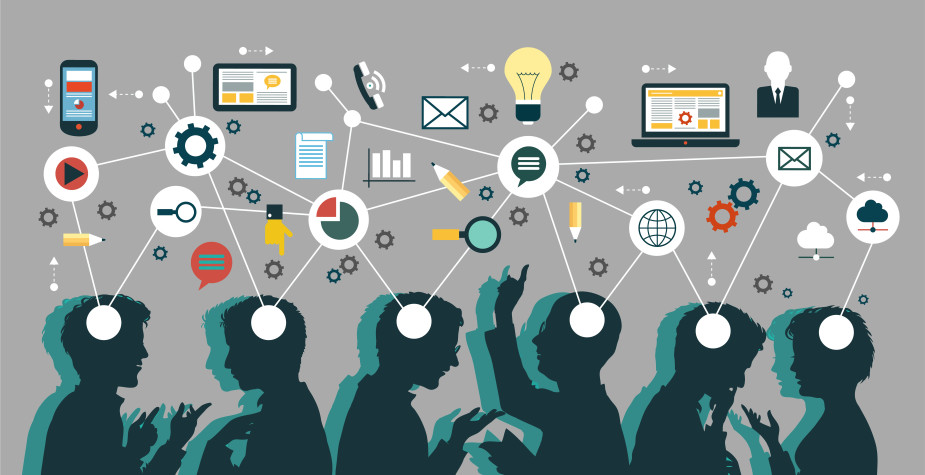
\includegraphics[scale = 1.0]{Figuras/Conectados-pela-internet.jpg}
    \end{figure}

\end{frame}
%[Transparência 14] Garantindo cada um desses requisitos, munido de toda a infraestrutura de um governo eletrônico e contornados todos os empecilhos e demais questões a serem superada como: infraestrutura, e problemas sociais. Nós podemos em vias de fato alcançar a democracia eletrônica. Comigo, contigo, e com todos nós, podendo ser agentes ativos na participação na colaboração nas mudanças do nosso país. Trabalhando todos juntos, em uma sociedade unida através da internet, para a progressão e evolução do nosso país.


\begin{frame}
    \begin{center}
        \begin{figure}{\textit{"Democracy is the government of the people, by the people, for the people"}}
            \textit{ - Abraham Lincoln, 1864}
        \end{figure}
    \vspace{1.5cm}

    \begin{Huge} 
    Obrigado!\\
    \end{Huge}
    \bigskip
    Alexandre Mendonça Fava - \alert{alexandre.fava@hotmail.com}\\
    \end{center}
\end{frame}

\end{document}